\section{1174080 - Handi Hermawan}
\subsection{Soal Teori}
\begin{enumerate}

	\item Jelaskan kenapa file suara harus di lakukan MFCC. dilengkapi dengan ilustrasi atau gambar.
	\hfill\break
	Karena MFCC adalah koefisien yang mewakili audio. Machine learning tidak memahami rekaman suara melainkan vektor. Maka rekaman tersebut akan diubah kedalam bentuk vektor kemudian vektor akan menyesuaikan dengan kata kata yang sudah disediakan. Ekstraksi fitur dalam proses ini ditandai dengan konversi data suara menjadi gambar spektrum gelombang. File audio dilakukan oleh MFCC sehingga objek suara dapat dikonversi menjadi matriks. Suara akan menjadi vektor yang akan diproses sebagai output. Selain mempermudah mesin dalam bahasa ini karena mesin tidak dapat membaca teks, maka MFCC perlu mengubah suara menjadi vektor.  

	\begin{figure}[H]
	\centering
		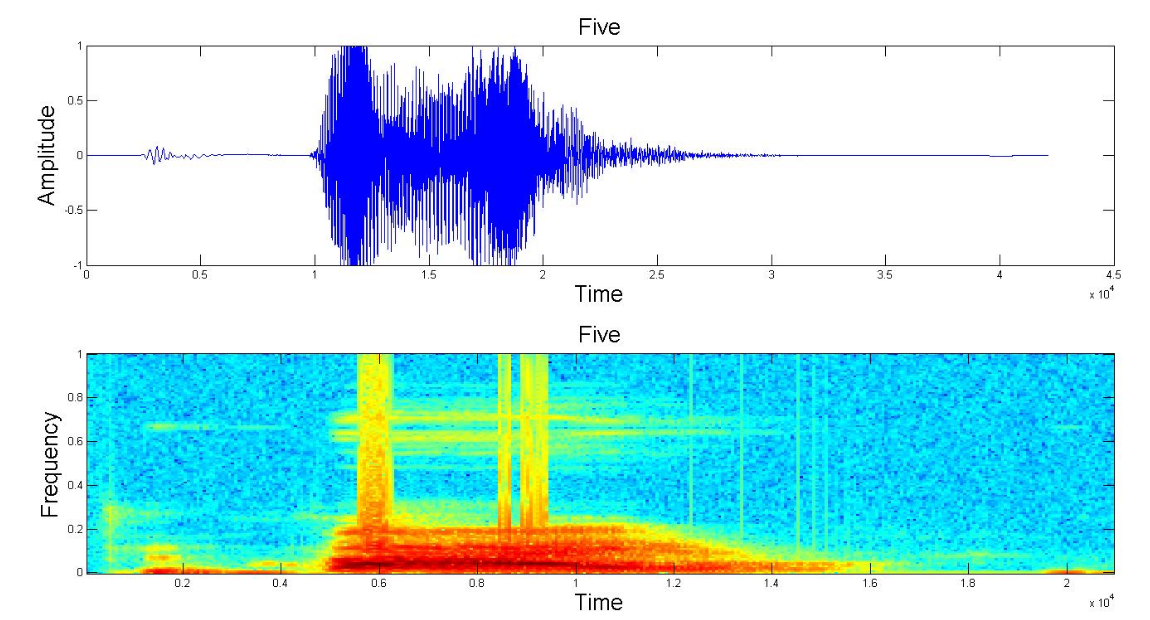
\includegraphics[width=4cm]{figures/1174080/6/materi/teori1.PNG}
		\caption{Teori 1}
	\end{figure}

	\item Jelaskan konsep dasar neural network.dilengkapi dengan ilustrasi atau gambar.
	\hfill\break
	Konsep sederhana dari neural network atau jaringan saraf sederhana dengan proses pembelajaran pada anak-anak dengan memetakan pola-pola baru yang diperoleh dari input untuk membuat pola-pola baru pada output. Contoh sederhana ini menganalogikan kinerja otak manusia. Jaringan saraf itu sendiri terdiri dari unit pemrosesan yang disebut neuron yang berisi fungsi adder dan aktivasi. Fungsi aktivasi itu sendiri untuk publikasi diberikan oleh neuron. Jaringan saraf yang mendukung pemikiran sistem atau aplikasi yang melibatkan otak manusia, baik untuk mendukung berbagai elemen sinyal yang diterima, memeriksa kesalahan, dan juga memproses secara paralel. Karakteristik neural network atau jaringan saraf dilihat dari pola hubungan antar neuron, metode penentuan bobot setiap koneksi, dan fungsi aktivasi mereka..  

	\begin{figure}[H]
	\centering
		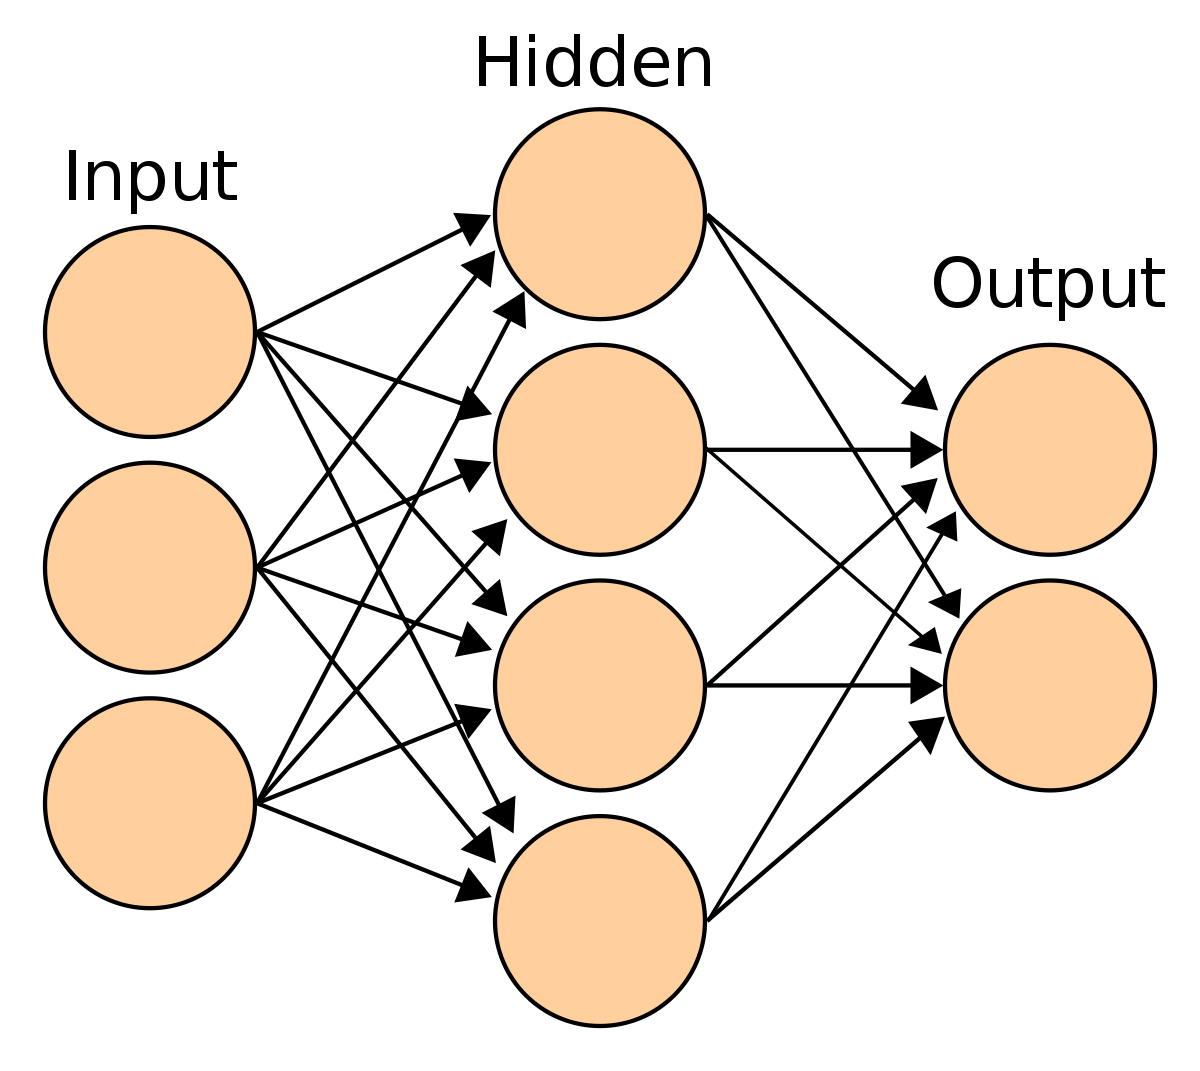
\includegraphics[width=4cm]{figures/1174080/6/materi/teori2.PNG}
		\caption{Teori 2}
	\end{figure}
	
	\item Jelaskan konsep pembobotan dalam neural network.dilengkapi dengan ilustrasi atau gambar.
	\hfill\break
	Pembobotan di dalam neural network juga akan menentukan penanda konektivitas. Dalam proses neural network mulai dari input yang diterima oleh neuron bersama dengan nilai bobot masing-masing input. Setelah memasuki neuron, nilai input akan ditambahkan oleh fungsi penerima. Hasil penambahan ini akan diproses oleh masing-masing fungsi neuron, hasil penambahan ini akan dibandingkan dengan nilai ambang tertentu. Jika nilai jumlah ini melebihi nilai ambang batas, aktivasi neuron akan dibatalkan, tetapi sebaliknya jika jumlah hasil di bawah nilai ambang batas, neuron akan diaktifkan. Setelah neuron aktif maka akan mengirimkan nilai output melalui bobot outputnya ke semua neuron yang terkait.  

	\begin{figure}[H]
	\centering
		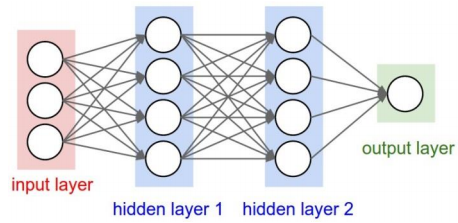
\includegraphics[width=4cm]{figures/1174080/6/materi/teori3.PNG}
		\caption{Teori 3}
	\end{figure}

	\item Jelaskan konsep fungsi aktifasi dalam neural network. dilengkapi dengan ilustrasi atau gambar.
	\hfill\break
	Fungsi aktivasi dalam neural network ialah merupakan suatu operasi matematik yang dikenakan pada sinyal output. Fungsi ini digunakan untuk mengaktifkan atau menonaktifkan neuron. Fungsi aktivasi ini terbagi setidaknya menjadi 6, adapun sebagai berikut:
	\begin{itemize}
	\item Fungsi Undak Biner Hard Limit, fungsi ini biasanya digunakan oleh jaringan lapiran tunggal untuk mengkonversi nilai input dari suatu variabel yang bernilai kontinu ke suatu nilai output biner 0 atau 1.
	\item Fungsi Undak Biner Threshold, fungsi ini menggunakan nilai ambang sebagai batasnya.
	\item Fungsi Bipolar Symetric Hard Limit, fungsi ini memiliki output bernilai 1, 0 atau -1.
	\item Fungsi Bipolar dengan Threshold, fungsi ini mempunyai output yang bernilai 1, 0 atau -1 untuk batas nilai ambang tertentu.
	\item Fungsi Linear atau Identitas.
	\end{itemize}. 
	Namun, untuk ilustrasi lihat gambar berikut: 

	\begin{figure}[H]
	\centering
		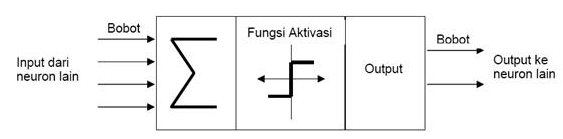
\includegraphics[width=4cm]{figures/1174080/6/materi/teori4.PNG}
		\caption{Teori 4}
	\end{figure}

	\item Jelaskan cara membaca hasil plot dari MFCC,dilengkapi dengan ilustrasi atau gambar
	\hfill\break
	Penelitian ini dilakukan untuk mengatahui  hasil dari ekstraksi ciri MFCC dari ucapan emosi manusia. Penelitian ini mengunakan software Matlab R2013a dengan menggunakan sampel dari ucapan aktor di database Berlin Database of Emotional. Bahasa yang digunakan adalah bahasa Berlin. Metode MFCC dalam penelitian ini digunakan untuk mengekstraksi ciri sampel ucapan dari aktor. Berikut adalah langkah-langkah tahapan penelitian:

	\begin{figure}[H]
	\centering
		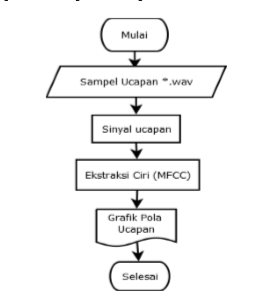
\includegraphics[width=4cm]{figures/1174080/6/materi/teori5.PNG}
		\caption{Teori 5}
	\end{figure}

	\item Jelaskan apa itu one-hot encoding,dilengkapi dengan ilustrasi kode dan atau gambar.
	\hfill\break
	Digunakan dalam pembelajaran mesin sebagai metode untuk mengukur data kategorikal. Singkatnya, metode ini menghasilkan vektor dengan panjang yang sama dengan jumlah kategori dalam kumpulan data. Jika titik data milik kategori engan maka komponen dari vektor ini diberi nilai 0 kecuali untuk komponen engan, yang diberi nilai 1. Dengan cara ini seseorang dapat melacak kategori dengan cara yang bermakna secara numerik. Mungkin timbul pertanyaan: Apa yang terjadi jika ada banyak 1? Klasifikasi mana yang benar? Ini dengan cepat diperbaiki oleh fakta bahwa sesuatu yang dikodekan satu-panas memiliki tepat satu posisi dalam array yang diberi label sebagai 1. Misalnya, [0,0,0,1,0] akan menjadi satu-panas yang valid pengkodean yang akan memberitahu Anda klasifikasi di posisi 4 (atau 3 dalam pengindeksan array) adalah klasifikasi objek. Sebaliknya, [0,1,0,1,0], dan [1,1,1,1,1] adalah contoh pengkodean, seperti :

	\begin{figure}[H]
	\centering
		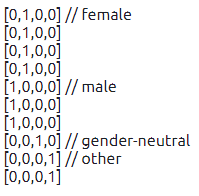
\includegraphics[width=4cm]{figures/1174080/6/materi/teori6_1.PNG}
		\caption{Teori 6}
	\end{figure}

	\item Jelaskan apa fungsi dari np.unique dan to categorical dalam kode program,dilengkapi dengan ilustrasi atau gambar.
	\hfill\break
	numpy.unique untuk mengembalikan elemen unik array yang diurutkan. Ada tiga output opsional selain elemen unik: indeks array input yang memberikan nilai unik dan indeks array unik yang merekonstruksi array input berapa kali setiap nilai unik muncul dalam array input

	\begin{figure}[H]
	\centering
		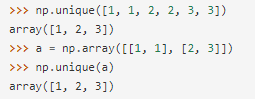
\includegraphics[width=4cm]{figures/1174080/6/materi/teori7_1.PNG}
		\caption{Teori 7}
	\end{figure}

	Fungsi dari to\_categorical ialah untuk mengubah suatu vektor yang berupa integer menjadi matrix dengan kelas biner. Untuk ilustrasinya bisa dilihat pada gambar untuk memproses categorical data kolom Country \ref{cc71}
		\begin{figure}[H]
	\centering
		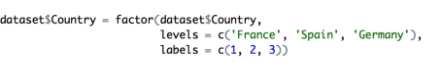
\includegraphics[width=4cm]{figures/1174080/6/materi/teori7_2.PNG}
		\caption{Teori 7}
	\end{figure}

	\item Jelaskan apa fungsi dari Sequential dalam kode program,dilengkapi dengan ilustrasi atau gambar.
	\hfill\break
	Fungsi dari Sequential sebagai salah satu jenis model yang digunakan dalam perhitungan. Sequential ini membangun tumpukan linear yang berurutan. Untuk ilusrasi gambar sebagai betikut : 

	\begin{figure}[H]
	\centering
		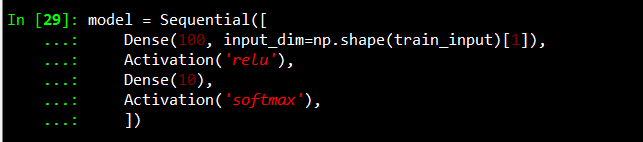
\includegraphics[width=4cm]{figures/1174080/6/materi/teori8.PNG}
		\caption{Teori 8}
	\end{figure}
\end{enumerate}

\subsection{Praktek Program}
\begin{enumerate}
	\item Soal 1
	\hfill\break
	\lstinputlisting[firstline=7, lastline=28]{src/1174080/6/1174080.py}
	Kode di atas menjelaskan isi data GTZAN. Ini adalah kumpulan data yang berisi 10 genre lagu dengan masing-masing genre memiliki 100 lagu yang akan kami lakukan proses MFCC dan juga freesound yang hanya berisi konten lagu, jika GTZAN memiliki beberapa genre jika freesound hanya untuk 1 lagu dan disini kita membuat fungsi untuk membaca file audio dan outputnya sebagai plot, hasilnya adalah sebagai berikut:
	\begin{figure}[H]
	\centering
		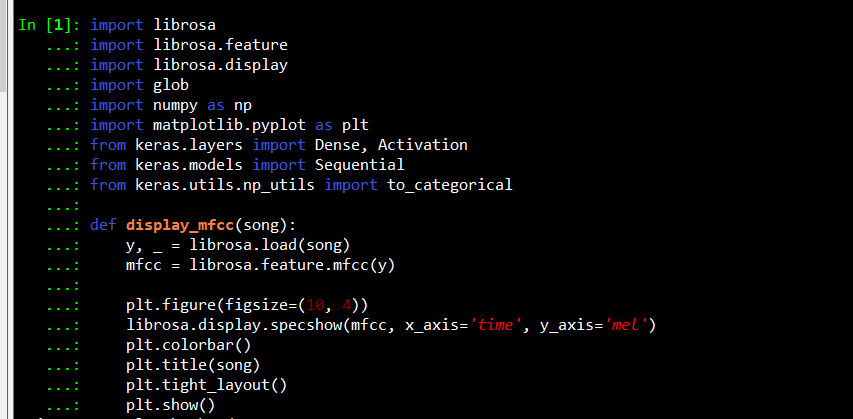
\includegraphics[width=4cm]{figures/1174080/6/materi/hasil1.PNG}
		\caption{Hasil Soal 1.}
	\end{figure}

	\item Soal 2
	\hfill\break
	\lstinputlisting[firstline=29, lastline=50]{src/1174080/6/1174080.py}
	Kode di atas akan menampilkan hasil dari proses mfcc yang sudah dibuat fungsi pada soal 1, yaitu display mfcc() dan akan menampilkan plot dari pembacaan file audio. Berikut adalah hasil setelah saya lakukan running dan pembacaan file audio :
	\begin{figure}[H]
	\centering
		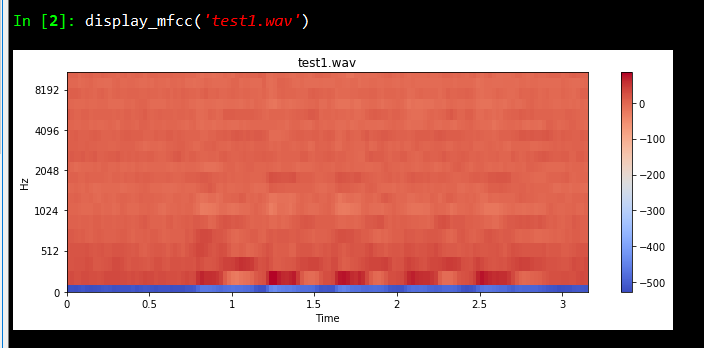
\includegraphics[width=4cm]{figures/1174080/6/materi/hasil2_1.PNG}
		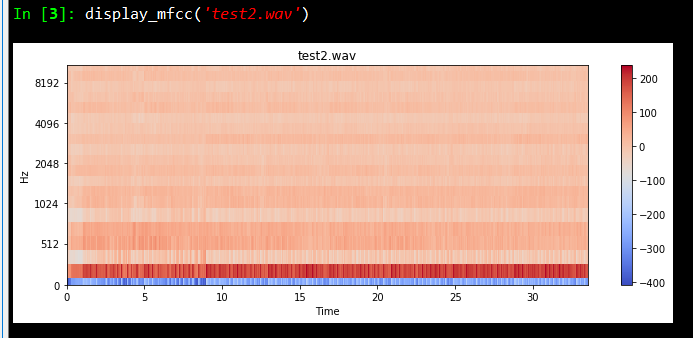
\includegraphics[width=4cm]{figures/1174080/6/materi/hasil2_2.PNG}
		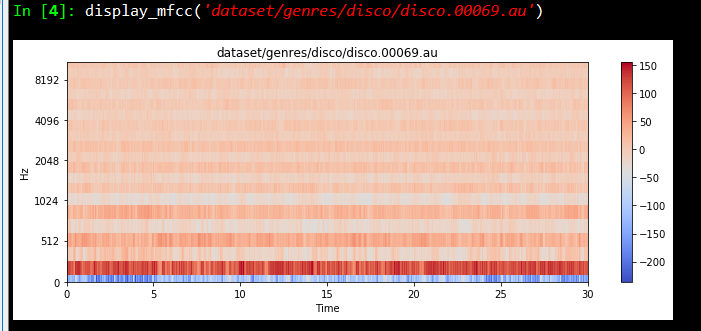
\includegraphics[width=4cm]{figures/1174080/6/materi/hasil2_3.PNG}
		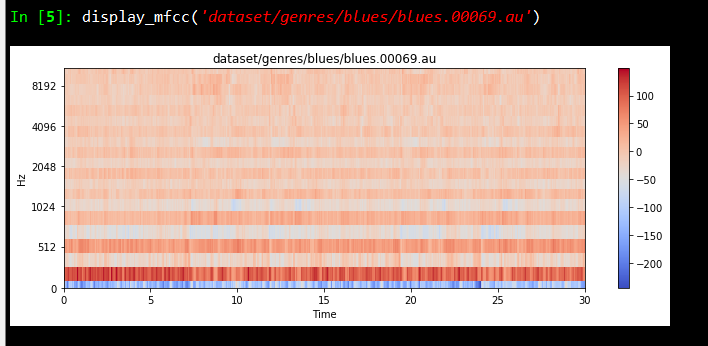
\includegraphics[width=4cm]{figures/1174080/6/materi/hasil2_4.PNG}
		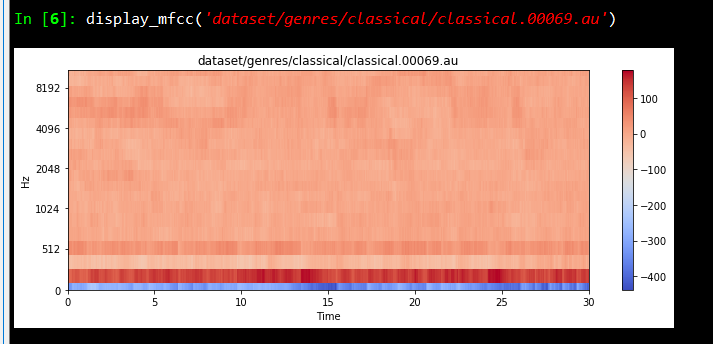
\includegraphics[width=4cm]{figures/1174080/6/materi/hasil2_5.PNG}
		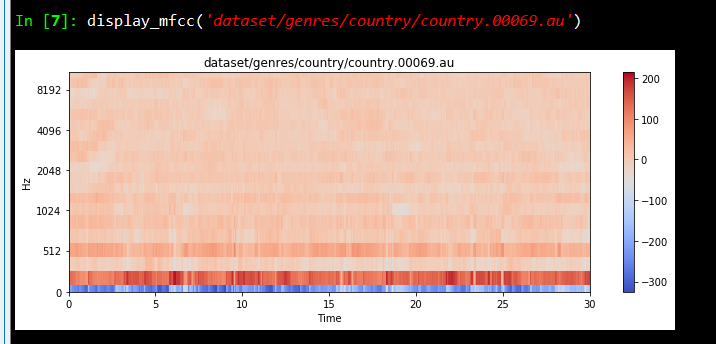
\includegraphics[width=4cm]{figures/1174080/6/materi/hasil2_6.PNG}
		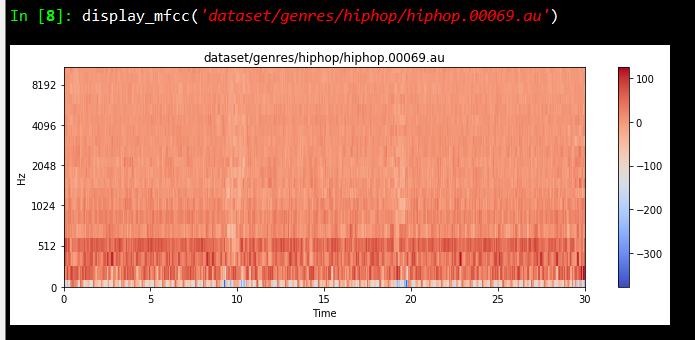
\includegraphics[width=4cm]{figures/1174080/6/materi/hasil2_7.PNG}
		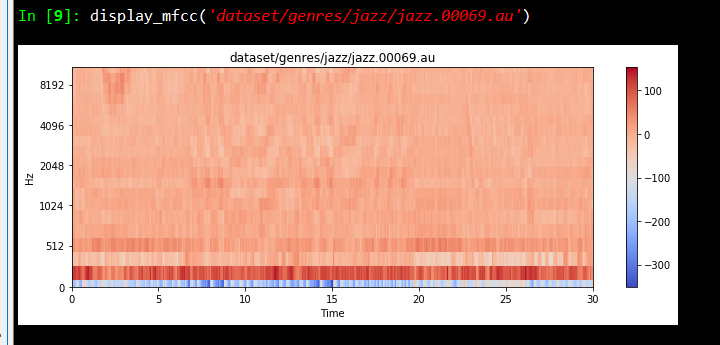
\includegraphics[width=4cm]{figures/1174080/6/materi/hasil2_8.PNG}
		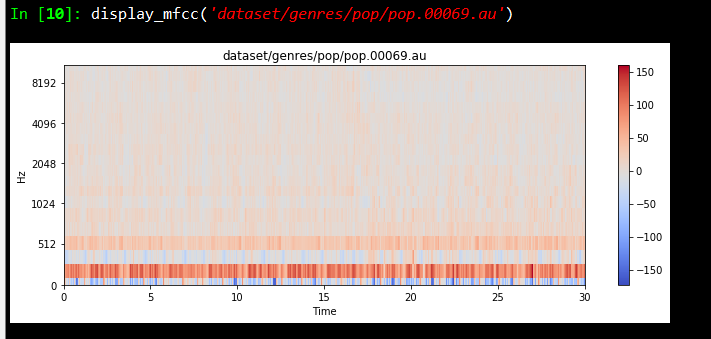
\includegraphics[width=4cm]{figures/1174080/6/materi/hasil2_9.PNG}
		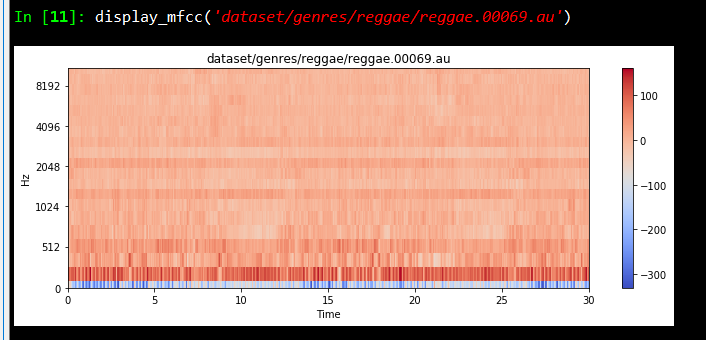
\includegraphics[width=4cm]{figures/1174080/6/materi/hasil2_10.PNG}
		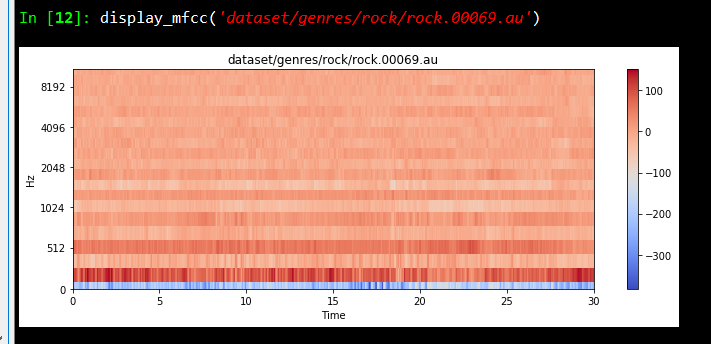
\includegraphics[width=4cm]{figures/1174080/6/materi/hasil2_11.PNG}
		\caption{Hasil Soal 2.}
	\end{figure}

	\item Soal 3
	\hfill\break
	\lstinputlisting[firstline=51, lastline=61]{src/1174080/6/1174080.py}
	Baris pertama itu untuk membuat fungsi extract\_features\_song(f). Pada baris kedua itu akan me-load data inputan dengan menggunakan librosa. Lalu selanjutnya untuk membuat sebuah fitur untuk mfcc dari y atau parameter inputan. Lalu akan me-return menjadi array dan akan mengambil 25000 data saja dari hasil vektorisasi dalam 1 lagu. Hasilnya adalah sebagai berikut :
	\begin{figure}[H]
	\centering
		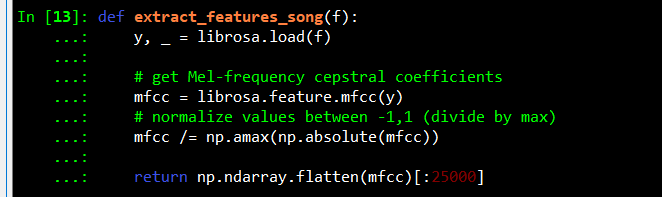
\includegraphics[width=4cm]{figures/1174080/6/materi/hasil3.PNG}
		\caption{Hasil Soal 3.}
	\end{figure}

	\item Soal 4
	\hfill\break
	\lstinputlisting[firstline=63, lastline=82]{src/1174080/6/1174080.py}
	Kode di atas dapat digunakan untuk melakukan fungsi yang sebelumnya telah kita lakukan. Kemudian di bagian genre yang disesuaikan dengan dataset nama folder. Untuk baris berikutnya akan mengulang genre folder dengan ekstensi .au. Maka itu akan memanggil fungsi ekstrak lagu. Setiap file dalam folder itu akan diekstraksi menjadi vektor dan akan ditambahkan ke fitur. Dan fungsi yang ditambahkan adalah untuk menumpuk file yang telah di-vektor-kan. Hasil kode tidak menampilkan output. Hasilnya adalah sebagai berikut :
	\begin{figure}[H]
	\centering
		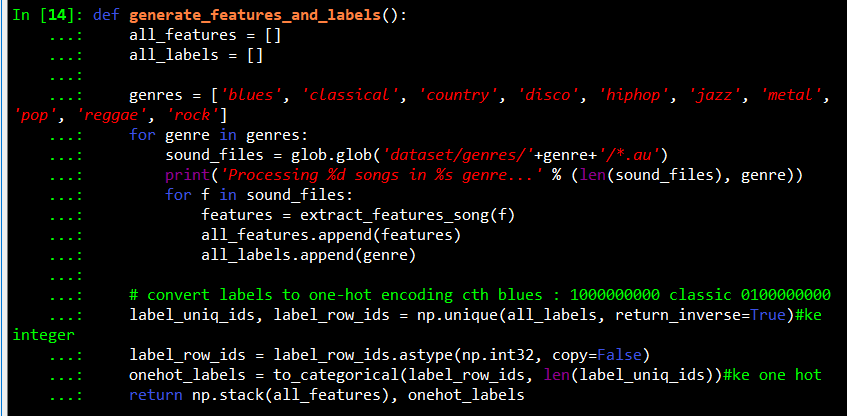
\includegraphics[width=4cm]{figures/1174080/6/materi/hasil4.PNG}
		\caption{Hasil Soal 4.}
	\end{figure}

	\item Soal 5
	\hfill\break
	\lstinputlisting[firstline=84, lastline=89]{src/1174080/6/1174080.py}
	Kode diatas berfungsi untuk melakukan load variabel features dan labels. Mengapa memakan waktu yang lama ? Karena mesin akan melakukan vektorisasi terhadap semua file yang berada pada setiap foldernya, di sini terdapat 10 folder dengan masing-masing folder terdiri atas 100 buah lagu, setiap lagu tersebut akan dilakukan vektorisasi atau ekstraksi data menggunakan mfcc. Oleh karena itu, proses cukup memakan waktu. Hasilnya adalah sebagai berikut :
	\begin{figure}[H]
	\centering
		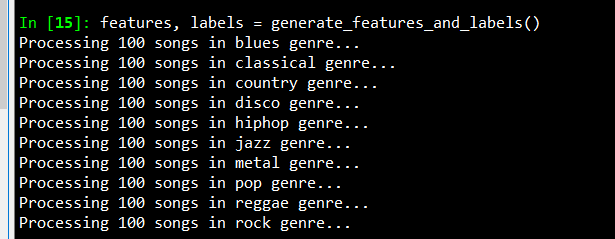
\includegraphics[width=4cm]{figures/1174080/6/materi/hasil5_1.PNG}
		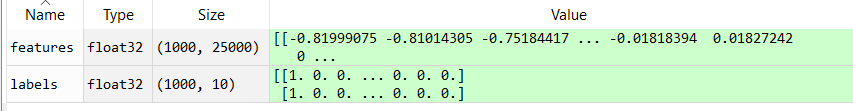
\includegraphics[width=4cm]{figures/1174080/6/materi/hasil5_2.PNG}
		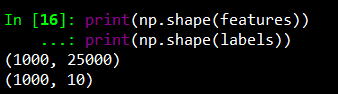
\includegraphics[width=4cm]{figures/1174080/6/materi/hasil5_3.PNG}
		\caption{Hasil Soal 5.}
	\end{figure}

	\item Soal 6
	\hfill\break
	\lstinputlisting[firstline=90, lastline=109]{src/1174080/6/1174080.py}
	Kode diatas berfungsi untuk melakukan training split 80\%. Karena supaya mesin dapat terus belajar tentang data baru, jadi ketika prediksi dibuat tentang data yang terlatih itu bisa mendapatkan persentase yang cukup bagus. Hasilnya adalah sebagai berikut :
	\begin{figure}[H]
	\centering
		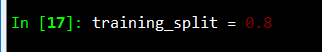
\includegraphics[width=4cm]{figures/1174080/6/materi/hasil6_1.PNG}
		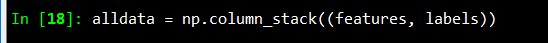
\includegraphics[width=4cm]{figures/1174080/6/materi/hasil6_2.PNG}
		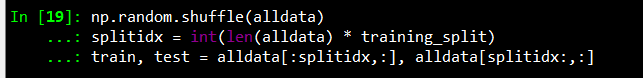
\includegraphics[width=4cm]{figures/1174080/6/materi/hasil6_3.PNG}
		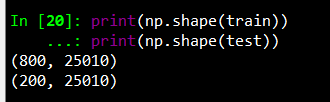
\includegraphics[width=4cm]{figures/1174080/6/materi/hasil6_4.PNG}
		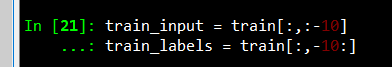
\includegraphics[width=4cm]{figures/1174080/6/materi/hasil6_5.PNG}
		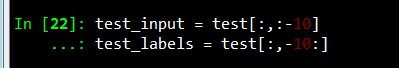
\includegraphics[width=4cm]{figures/1174080/6/materi/hasil6_6.PNG}
		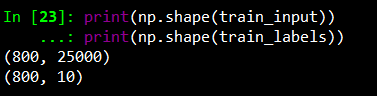
\includegraphics[width=4cm]{figures/1174080/6/materi/hasil6_7.PNG}
		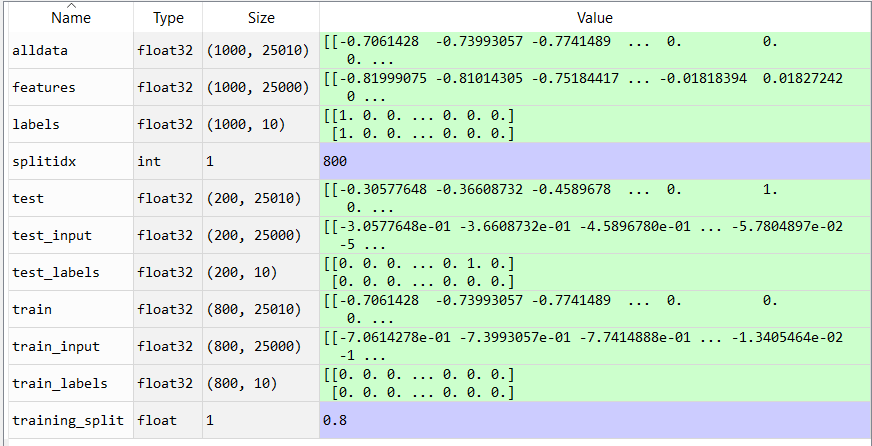
\includegraphics[width=4cm]{figures/1174080/6/materi/hasil6_8.PNG}
		\caption{Hasil Soal 6.}
	\end{figure}

	\item Soal 7
	\hfill\break
	\lstinputlisting[firstline=111, lastline=117]{src/1174080/6/1174080.py}
	fungsi Sequential() ialah Sebuah model untuk menentukan izin pada setiap neuron, di sini adalah 100 dense yang merupakan 100 neuron pertama dari data pelatihan. Fungsi dari relay itu sendiri adalah untuk mengaktifkan neuron atau input yang memiliki nilai maksimum. Sedangkan untuk dense 10 itu adalah output dari hasil neuron yang telah berhasil diaktifkan, untuk dense 10 diaktifkan menggunakan softmax. Hasilnya adalah sebagai berikut :
	\begin{figure}[H]
	\centering
		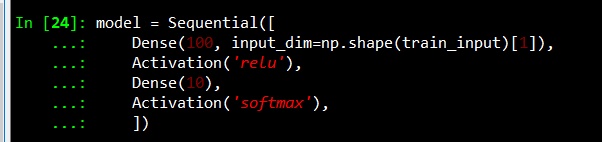
\includegraphics[width=4cm]{figures/1174080/6/materi/hasil7.PNG}
		\caption{Hasil Soal 7.}
	\end{figure}

	\item Soal 8
	\hfill\break
	\lstinputlisting[firstline=118, lastline=122]{src/1174080/6/1174080.py}
	Model Compile di perjelas dengan gambar dibawah, Hasil output pada kode tersebut seperti gambar  menjelaskan bahwa dense pertama itu memiliki 100 neurons dengan parameter sekitar 2 juta lebih dengan aktviasi 100, jadi untuk setiap neurons memiliki masing-masing 1 aktivasi. Sama halnya seperti dense 2 memiliki jumlah neurons sebanyak 10 dengan parameter 1010 dan jumlah aktivasinya 10 untuk setiap neurons tersebut dan total parameternya sekitar 2.5 juta data yang akan dilatih pada mesin tersebut.
	\begin{figure}[H]
	\centering
		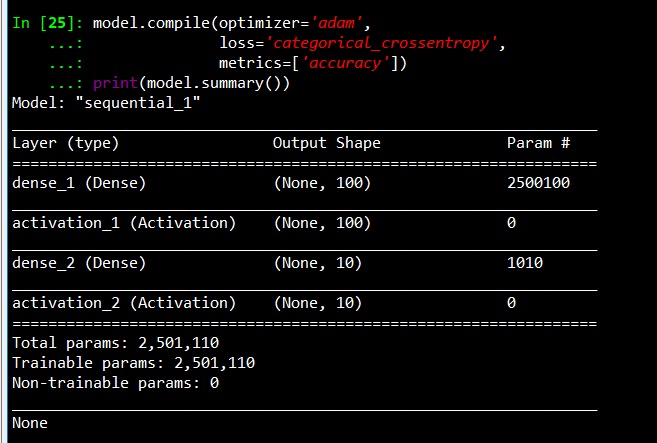
\includegraphics[width=4cm]{figures/1174080/6/materi/hasil8.PNG}
		\caption{Hasil Soal 8.}
	\end{figure}

	\item Soal 9
	\hfill\break
	\lstinputlisting[firstline=123, lastline=125]{src/1174080/6/1174080.py}
	Kode tersebut berfungsi untuk melatih mesin dengan data training input dan training label. Epochs ini merupakan iterasi atau pengulangan berapa kali data tersebut akan dilakukan. Batch\_size ini adalah jumlah file yang akan dilakukan pelatihan pada setiap 1 kali pengulangan. Sedangkan validation\_split itu untuk menentukan presentase dari cross validation atau k-fold sebanyak 20\% dari masing-masing data pengulangan, hasilnya adalah sebagai berikut :
	\begin{figure}[H]
	\centering
		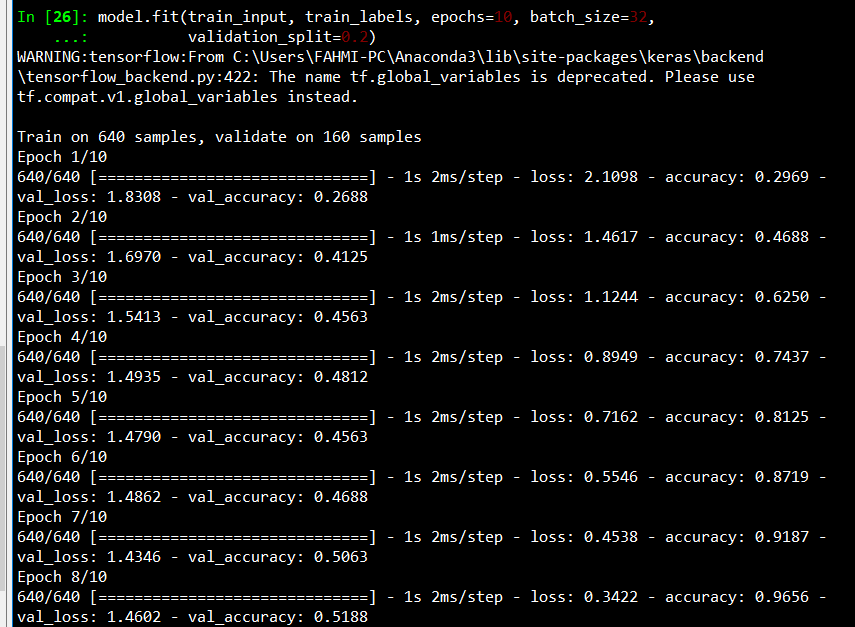
\includegraphics[width=4cm]{figures/1174080/6/materi/hasil9.PNG}
		\caption{Hasil Soal 9.}
	\end{figure}

	\item Soal 10
	\hfill\break
	\lstinputlisting[firstline=126, lastline=130]{src/1174080/6/1174080.py}
	Fungsi evaluate atau evaluasi ini ialah untuk menguji data pengujian setiap file. Di sini ada prediksi yang hilang, artinya mesin memprediksi data, sedangkan untuk keseluruhan perjanjian sekitar 55\%, hasilnya adalah sebagai berikut :
	\begin{figure}[H]
	\centering
		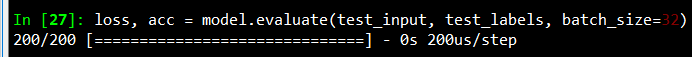
\includegraphics[width=4cm]{figures/1174080/6/materi/hasil10_1.PNG}
		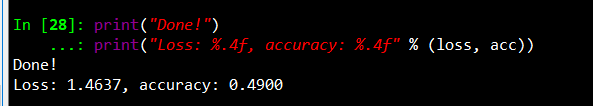
\includegraphics[width=4cm]{figures/1174080/6/materi/hasil10_2.PNG}
		\caption{Hasil Soal 10.}
	\end{figure}

	\item Soal 11
	\hfill\break
	\lstinputlisting[firstline=132, lastline=133]{src/1174080/6/1174080.py}
	Fungsi Predict ialah untuk menghasilkan suatu nilai yang sudah di prediksi dari data training sebelumnya. Gambar dibawah ini menjelaskan file yang di jalankan tersebut termasuk ke dalam genre apa, hasilnya bisa dilihat pada gambar tersebut presentase yang paling besar yakni genre rock. Maka lagu tersebut termasuk ke dalam genre rock dengan perbandingan presentase hasil prediksi.
	\begin{figure}[H]
	\centering
		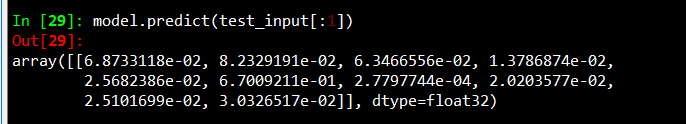
\includegraphics[width=4cm]{figures/1174080/6/materi/hasil11.PNG}
		\caption{Hasil Soal 11.}
	\end{figure}
\end{enumerate}

\subsection{Penanganan Error}
\begin{enumerate}
	\item ScreenShoot Error
	\begin{figure}[H]
		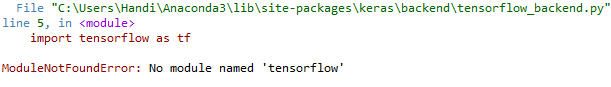
\includegraphics[width=4cm]{figures/1174080/6/error/1.PNG}
		\centering
		\caption{ModuleNotFoundError}
	\end{figure}

	\begin{figure}[H]
		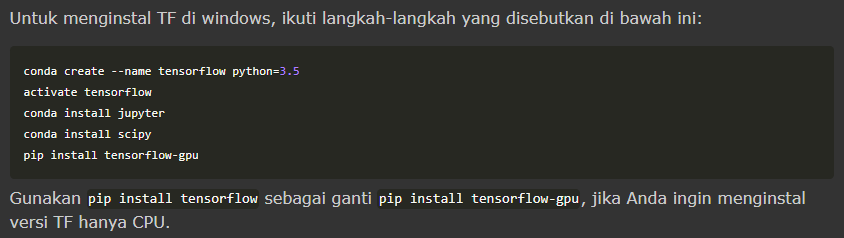
\includegraphics[width=4cm]{figures/1174080/6/error/2.PNG}
		\centering
		\caption{An error ocurred while starting the kernel}
	\end{figure}

	\item Cara Penanganan Error
	\begin{itemize}
		\item ModuleNotFoundError
		\hfill\break
		Error terdapat pada library yang tidak terbaca, karena library tensorflow belum di install, solusinya dengan menginstall library tersebut, pip install tensorflow.
		\item An error ocurred while starting the kernel
		\hfill\break
		Seperti pada gambar tersebut untuk mengistall tensorflow
	\end{itemize}
\end{enumerate}

\subsection{Bukti Tidak Plagiat}
\begin{figure}[H]
\centering
	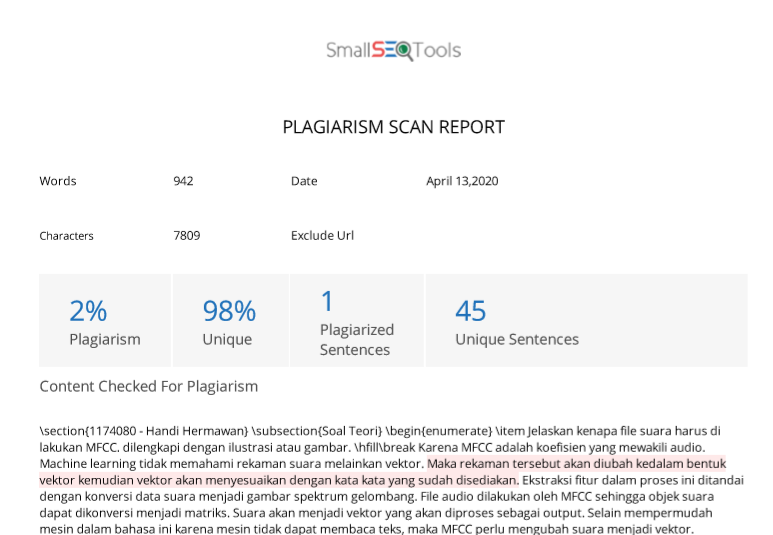
\includegraphics[width=4cm]{figures/1174080/6/materi/plagiat.PNG}
	\caption{Bukti Tidak Melakukan Plagiat Chapter 6}
\end{figure}

\subsection{Link Video Youtube}
https://youtu.be/MzxIZ-C-gi0